\chapter{Практическая часть}\label{ch:ch3}

\section{Система навигации робота}\label{sec:ch3/sect1}
Исходя из требований и выбранной среды выполнения, необходимо подготовить систему навигации робота, которая будет исполнять приказы нейронной сети с максимально возможной точностью и быстродействием. Для успешной навигации понадобится:
\begin{enumerate}[beginpenalty=10000] % https://tex.stackexchange.com/a/476052/104425
  \item Возможность регулирования скорости и направления движения для всех двух двигателей робота;
  \item Некоторая метрика, определяющая реальное пройденное роботом расстояние;
  \item Интеграция данной системы с Robot Operating System.
\end{enumerate}

\subsection{ROS Navigation Stack}
В ROS уже есть готовые и по большей части универсальные реализации систем навигации: они подойдут для большого количества нужд. Эта система навигации состоит из следующих компонентов:

\begin{enumerate}[beginpenalty=10000] % https://tex.stackexchange.com/a/476052/104425
  \item Transform или местоположение всех компонентов навигации;
  \item Измеритель пройденного пути или одометрия\footnote{подробнее об одометрии можно прочитать в разделе~\cref{sec:odom}};
  \item Контроллер двигателей;
  \item Планировщики путей;
  \item Узел картографирования (не обязательный компонент);
  \item Данные с датчиков для сбора информации о текущем состоянии.
\end{enumerate}

Схематично компоненты показаны на Рисунке~\cref{fig:nav-stack}~\cite{nav-stack}.

\begin{figure}[ht]
    \centerfloat{
        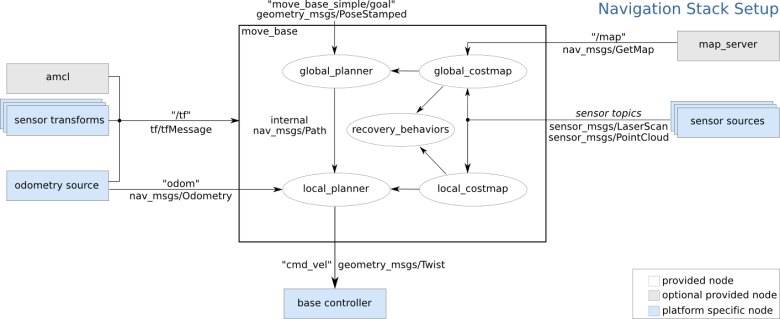
\includegraphics[scale=0.75]{nav-stack}
    }
    \caption{Компоненты ROS Navigation Stack}\label{fig:nav-stack}
\end{figure}

Стек навигации довольно прост на концептуальном уровне. Он принимает информацию из одометрии и датчиков, позволяя обрабатывать команды движения для отправки на драйвер двигателей. Однако использование навигационного стека на практике немного сложнее. В качестве предварительного условия для использования навигационного стека робот должен работать под управлением ROS, иметь дерево местоположений transform и публиковать данные с установленных датчиков, используя заранее оговоренные типы сообщений в ROS. Кроме того, навигационный стек необходимо настраивать для каждого конкретного робота, чтобы он мог работать на высоком уровне~\cite{nav-stack}.

Для реализации этой системы на данном роботе необходимо подготовить инструментарий. Этому посвящён следующий пункт.

\subsection{Дополнения к роботу для реализации ROS Navigation Stack}
В главе~\cref{ch:ch2} были описаны необходимые инструменты для функционирования нейронной сети, но этого недостаточно для запуска ROS Navigation Stack. Дополнительно понадобится возможность регулирования оборотов двигателей посредством использования интерфейсов, предоставляемых компьютером NVIDIA Jetson Xavier NX, а также подсчёт расстояния, пройденного роботом. 

Для регулирования оборотов двигателя было решено использовать устройство, которое называют драйвером двигателя. Его суть заключается в преобразовании цифровой команды на движение в конкретный электрический сигнал для двигателя. По сути драйвер будет являться посредником между компьютером и двигателями. К драйверу предъявляются следующие требования:

\begin{enumerate}[beginpenalty=10000] % https://tex.stackexchange.com/a/476052/104425
  \item Интерфейс управления должен быть совместим с компьютером;
  \item Устройство должно иметь маленькие габариты для установки на мобильного робота;
  \item Схема драйвера должна иметь совместимость с двигателями, установленных на шасси.
\end{enumerate}

\subsubsection{Одометрия} \label{sec:odom}
Для подсчёта расстояния, пройденного роботом использована одометрия. Одометрия - использование данных о движении приводов, для оценки перемещения. Мотивацией для подключения одометрии: необходимость получать информацию о фактических оборотах двигателей робота, так как по каким-либо физическим причинам она может отличаться от ожидаемой.

Для подсчёта фактических оборотов могут использоваться датчики Холла, схематично они изображённые на Рисунке~\cref{fig:hole}~\cite{hole}. Выходными данными данных датчиков является электрический импульс при прохождении колесом двигателя определённой точки~\cite[с. 265]{hole-book}.

\begin{figure}[ht]
    \centerfloat{
        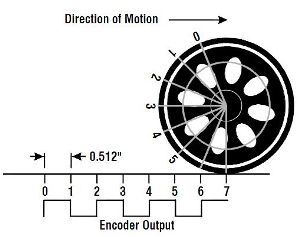
\includegraphics[scale=1.2]{hole}
    }
    \caption{Принцип работы датчиков Холла}\label{fig:hole}
\end{figure}

Подключение датчиков Холла было выполнено во встроенный в компьютер NVIDIA Jetson Xavier NX разъём GPIO с настройкой на приём входных данных на определённых ножках разъёма. Это подключение можно увидеть на Рисунке~\cref{fig:gpio-wire}.

\begin{figure}[ht]
    \centerfloat{
        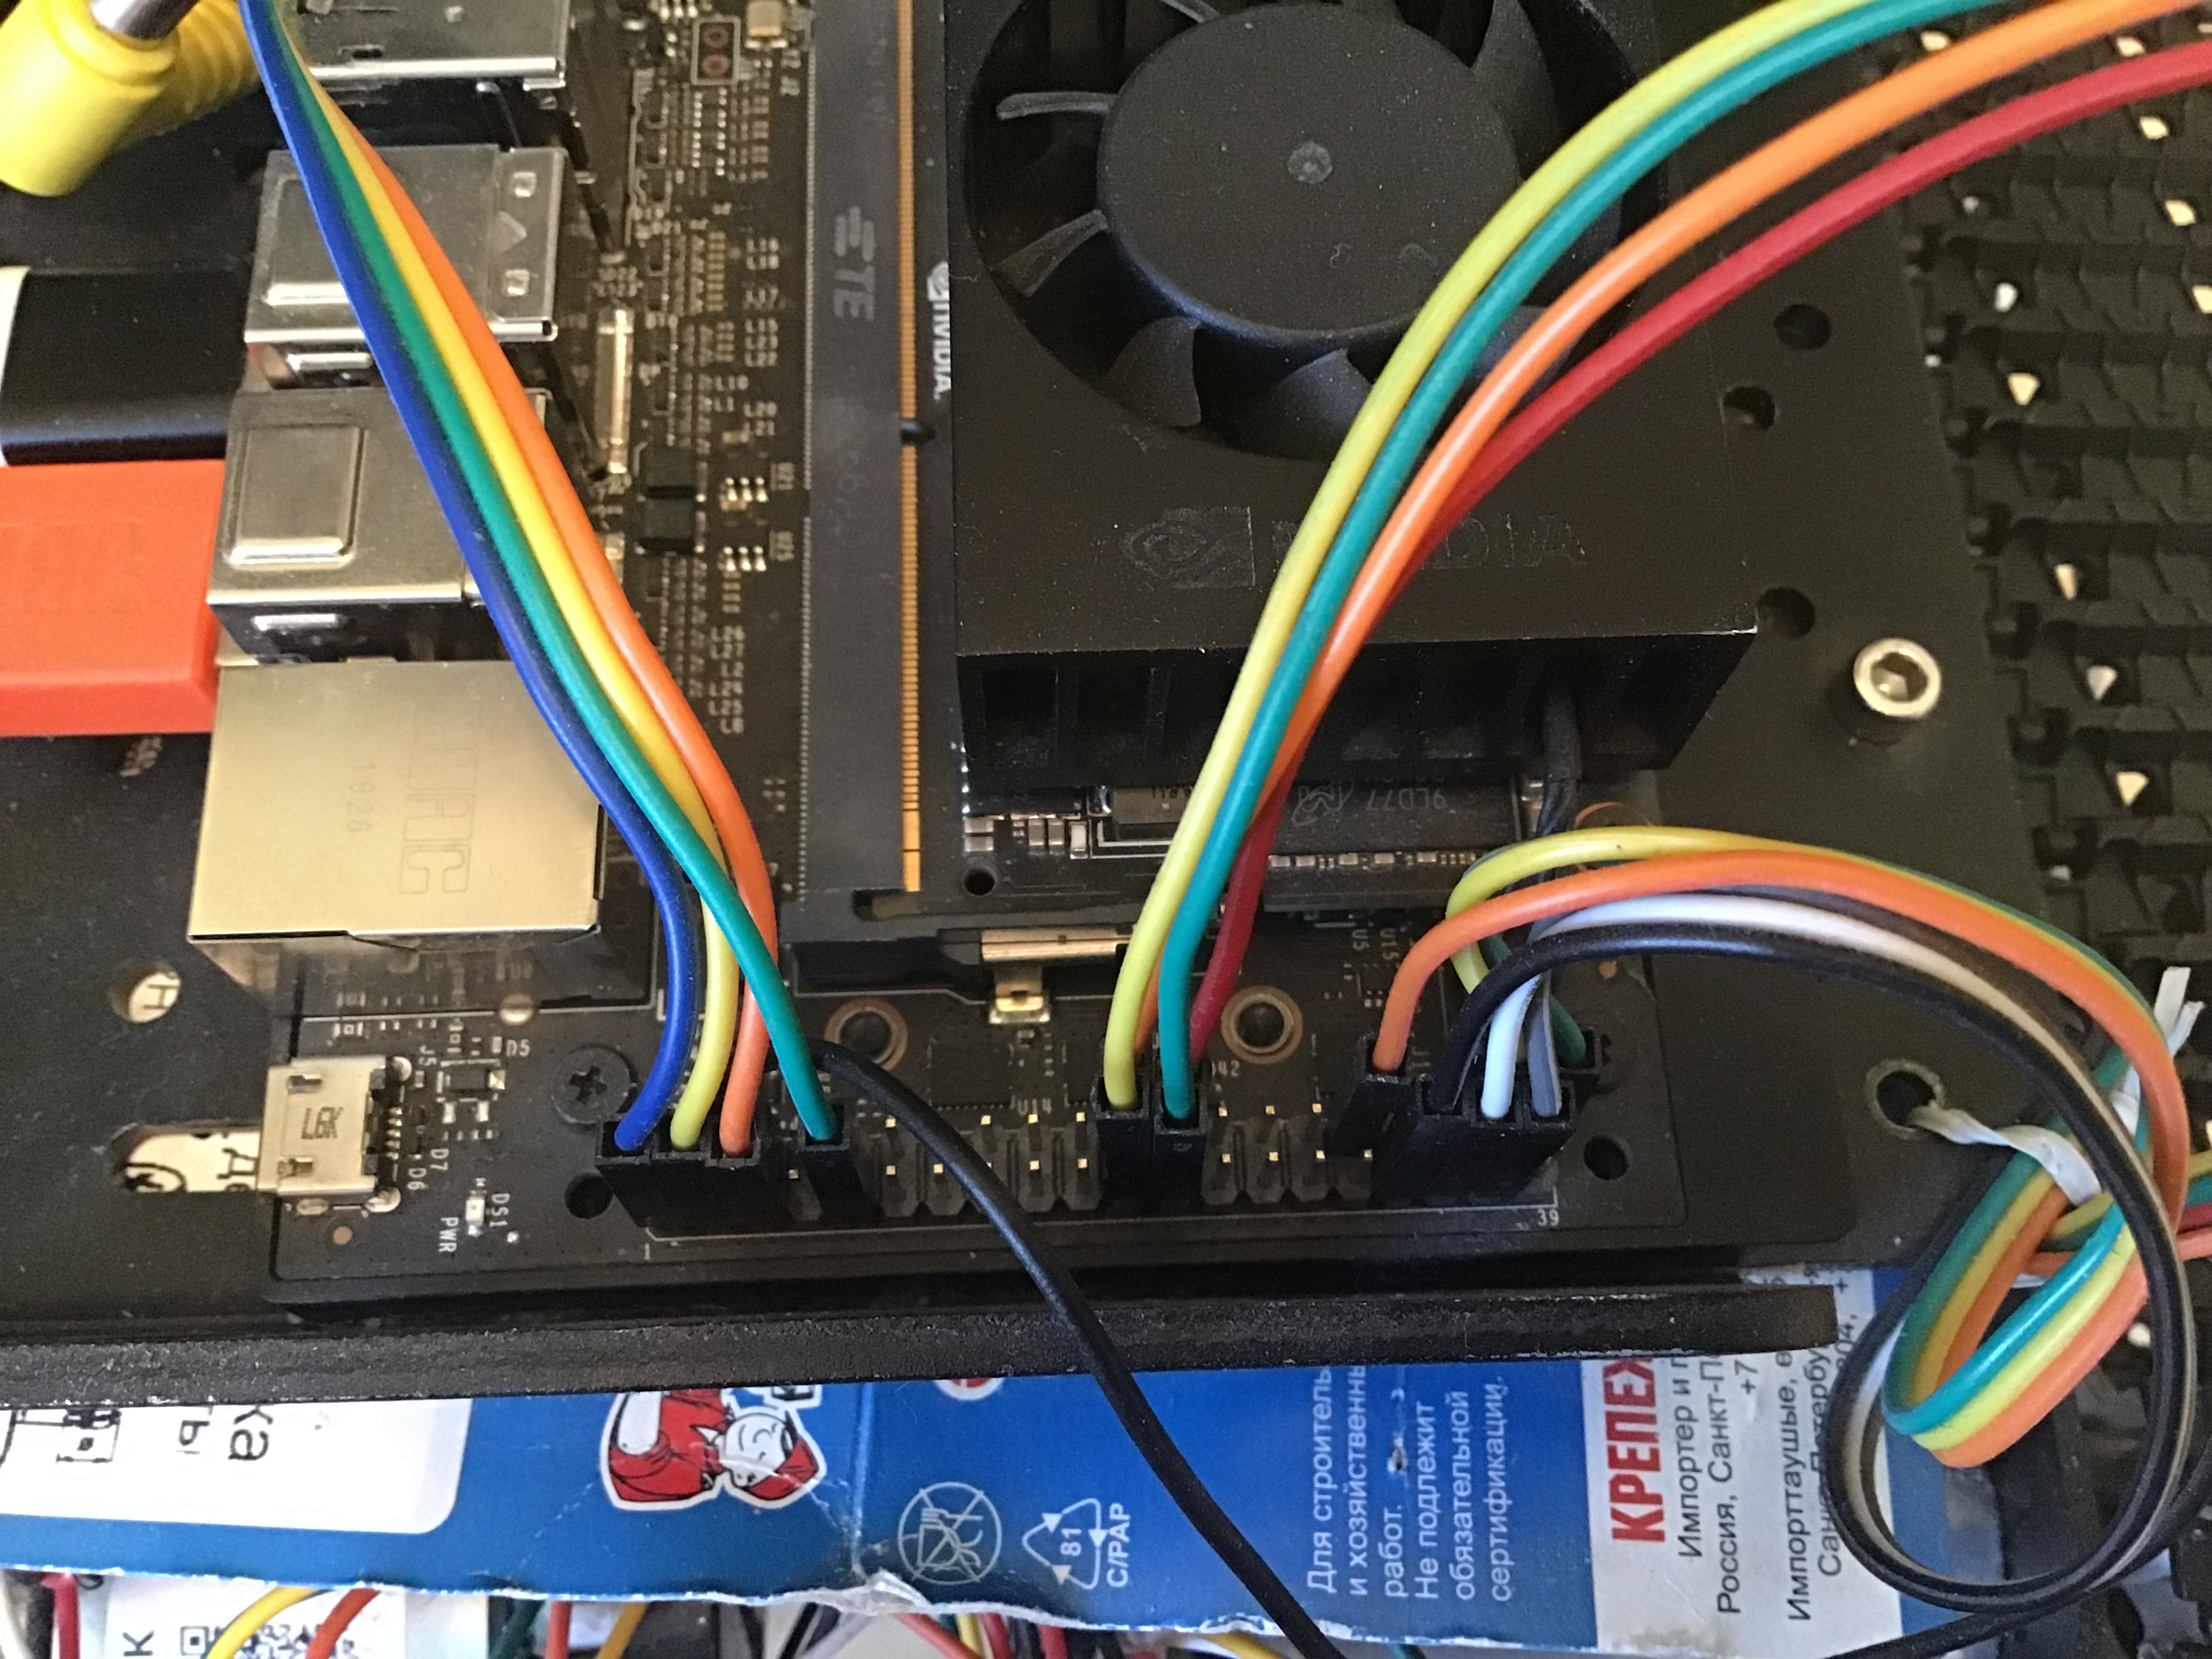
\includegraphics[scale=0.1]{gpio-wire}
    }
    \caption{Датчики Холла и драйвер двигателя подключены к GPIO интерфейсу компьютера NVIDIA Jetson Xavier NX}\label{fig:gpio-wire}
\end{figure}

\subsection{Драйвер двигателя}
В качестве драйвера двигателя выступило устройство Adafruit FeatherWing №2927, изображённое на Рисунке~\cref{fig:adafruit}~\cite{adafruit}. Оно имеет совместимый с NVIDIA Jetson Xavier NX интерфейс I2C, является четырёхканальным, а также подходит по габаритам и электрическим характеристикам.

\begin{figure}[ht]
    \centerfloat{
        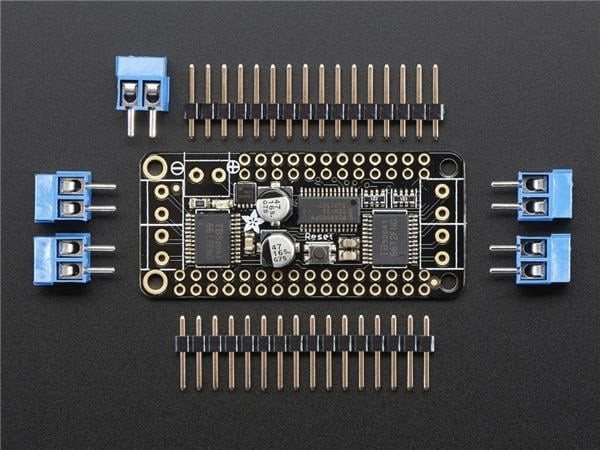
\includegraphics[scale=0.8]{adafruit}
    }
    \caption{Внешний вид драйвера Adafruit FeatherWing №2927.}\label{fig:adafruit}
\end{figure}

Данный драйвер может управлять, как двигателями постоянного тока, так и несколькими шаговыми двигателями. В дальнейшем, схему можно вертикально расширять, благодаря архитектуре серии продуктов Feather от Adafruit. Также стоит отметить следующие важные характеристики~\cite{adafruit}:

\begin{enumerate}[beginpenalty=10000] % https://tex.stackexchange.com/a/476052/104425
  \item Рабочее напряжение двигателей от 4.5 до 13.5 вольт;
  \item Максимальный ток на один канал 1.2 ампера;
  \item Для питания платы требуется напряжение 3.3 вольта.
\end{enumerate}

\subsection{Просчёт импульсов на GPIO}
Во время испытаний, которые проводились для реализации узлов ROS Navigation Stack, появились сомнения в точности одометрии робота. В испытаниях, проводимых на максимальной скорости движения робота были замечено, что импульсы сигнала с датчиков Холла на двигателях недосчитываются программой. Первые подозрения на недочёт легли на сами датчики. Данная гипотеза была проверена экспериментальным путём при помощи осциллографа. На Рисунке~\cref{fig:hole-signal} можно увидеть характерные для датчиков Холла импульсы. Их частота была стабильной и нареканий к работе датчиков вызвано не было.

\begin{figure}[ht]
    \centerfloat{
        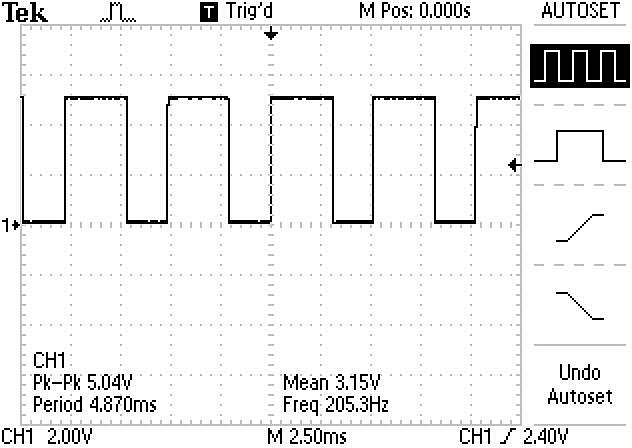
\includegraphics[scale=0.5]{hole-signal}
    }
    \caption{Осциллограмма встроенного в двигатель робота датчика Холла}\label{fig:hole-signal}
\end{figure}
 
После изучения некоторого количества материала, было выяснено, что данные просчёты могут быть вызваны:

\begin{enumerate}[beginpenalty=10000] % https://tex.stackexchange.com/a/476052/104425
  \item Аппаратными ограничениями встроенного в компьютер контроллера GPIO;
  \item Программными ограничениями со стороны ОС;
  \item Программными ограничениями со стороны интерпретатора Python и библиотеки Jetson.GPIO.
\end{enumerate}

Первый вариант был отсечён, так как компьютер аппаратно поддерживает чтение частоты импульсов до 50 кГц~\cite{gpio-limits}. Робот не двигается настолько быстро и частота его импульсов при наблюдениях не превышала 250 герц.

Второй вариант - это гипотеза о том, что ОС с разделением времени при достаточно высокой нагрузке не способна программно отследить все события изменения входного напряжения на ножке разъёма GPIO. Данный вариант представлен схематично на Рисунке~\cref{fig:miscount}.

\begin{figure}[ht]
    \centerfloat{
        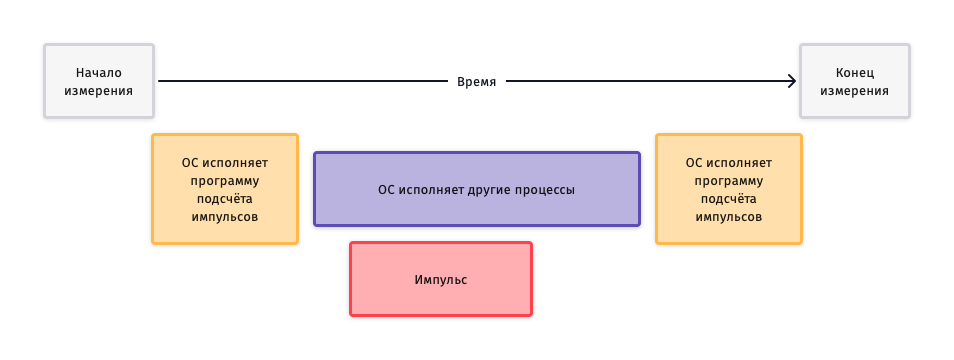
\includegraphics[scale=0.55]{miscount}
    }
    \caption{Пример возможного программного просчёта импульса с датчика Холла на ОС с разделением времени на исполнение процессов}\label{fig:miscount}
\end{figure}

Третий вариант - это не способность единственной написанной для платформы Jetson библиотеки для работы с GPIO, обеспечить достаточно быстрое чтение данных с аппаратной части в следствии не достаточно быстрой интерпретации и выполнения кода~\cite{gpio-limits}. Сам код, написанный для подсчёта импульсов представлен в Листинге~\cref{lst:encoders}.

Озвученные выше гипотезы не были доказаны, так как на исследование таких вопросов не было выделено достаточно времени. Вместо этого было предложено решать задачу подсчёта импульсов на внешнем устройстве.

\subsection{Микроконтроллер-посредник}
Для решения проблемы, описанной в пункте выше, было принято решение об установке некого посредника, способного подсчитывать импульсы энкодеров на аппаратном уровне, что позволит избежать таких просчётов. В качестве такого посредника был выбрана Arduino-совместимая платформа разработки Teensy 4.0, изображённая на Рисунке~\cref{fig:teensy}~\cite{teensy}.

\begin{figure}[ht]
    \centerfloat{
        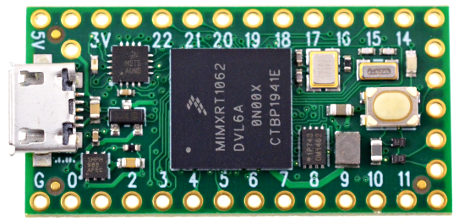
\includegraphics[scale=0.6]{teensy}
    }
    \caption{Внешний вид платформы Teensy 4.0}\label{fig:teensy}
\end{figure}

Среди ключевых особенностей данной платформы можно выделить следующие~\cite{teensy}:
\begin{itemize}[beginpenalty=10000] % https://tex.stackexchange.com/a/476052/104425
  \item Компактный форм-фактор 36x18x4~мм;
  \item ARM-процессор Cortex-M7 с таковой частотой 600 МГц;
  \item Оперативная память 1 МБ, встроенный Flash накопитель на 2 МБ;
  \item Широкий набор интерфейсов, показанных на Рисунке~\cref{fig:teensy-io}.
\end{itemize}

\begin{figure}[ht]
    \begin{minipage}[b][][b]{0.49\linewidth}\centering
        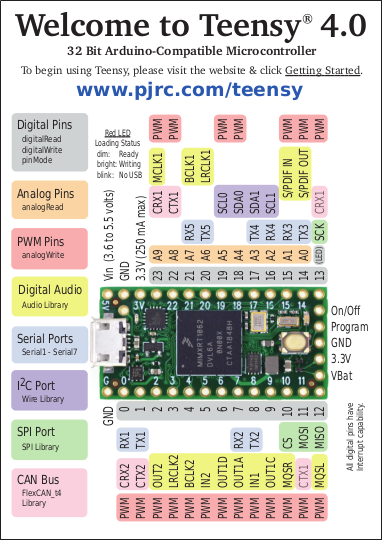
\includegraphics[width=\linewidth]{teensy-io1} \\ а)
    \end{minipage}
    \hfill
    \begin{minipage}[b][][b]{0.49\linewidth}\centering
        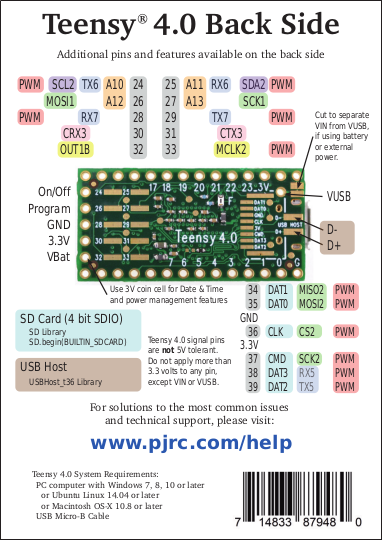
\includegraphics[width=\linewidth]{teensy-io2} \\ б)
    \end{minipage}
    \caption{Набор интерфейсов для подключения к платформе Teensy 4.0}
    \label{fig:teensy-io}
\end{figure}

\subsubsection{Коммуникация с внешним устройством}
Прошивка и коммуникация с платформой Teensy 4.0 осуществляется посредством USB подключения. Компьютер NVIDIA Jetson Xavier NX распознаёт устройство как последовательный серийный порт. Это позволит передавать между компьютером и платформой небольшое количество данных. В данном случае от этой платы требуется информация по подсчитанным с датчикам Холла импульсов. 

Для этих целей можно реализовать ROS узел, который по серийному порту будет выполнять коммуникацию с платформой Teensy, собирая с неё нужные данные. Такой способ вполне приемлем, однако есть более удобное решение, которое стало возможным благодаря обширной поддержке ROS, как самих Arduino совместимых платформ, так и встроенной возможности коммуникации в ROS. 

Данный способ представляет собой использование программы <<rosserial>>, которая занимается синхронизацией данных с подобными Arduino-совместимыми платформами нативным для ROS способом. Такой подход позволит использовать все преимущества фреймворка даже в коде прошивки на самой платформе Teensy, так как оба компьютера будут находиться в общем пространстве топиков и смогут читать/писать данные друг друга.

Единственное требование данного подхода - наличие запущенного сервера <<rosserial\_server>> на главном устройстве. В данном случае таким устройством будет выступать NVIDIA Jetson Xavier NX, а платформа Teensy 4.0 выступит клиентом, хотя на коде скетча это почти не отразится.

\subsubsection{Прошивка для платформы Teensy}
Для данной платформы была написана небольшая программа - скетч, который можно найти в Листинге~\cref{lst:impulse}, в котором происходит следующее:

\begin{enumerate}[beginpenalty=10000] % https://tex.stackexchange.com/a/476052/104425
  \item Инициализация объектов - сообщений о подсчитанных тиках для ROS и их публикатора;
  \item Подписка на специальный пустой топик <<reset>>, который сбрасывает счётчик подсчитанных импульсов;
  \item Считывание новых импульсов и публикация их в ROS топик <<encoder\_ticks>>; 
  \item Небольшой сон по команде <<delay(5)>>, который не позволяет переполниться буферу серийного порта.
\end{enumerate}

Основная проблема, которую предстояло решить - это формирование сообщения одометрии для ROS, которое можно найти в Листинге~\cref{lst:odom}\cite{odom}. Данную задачу удалось быстро решить благодаря обширному и активному сообществу ROS, которое на открытых площадках поделилось уже готовой реализацией ROS Hardware Interface - ряда пакетов, которые позволяют связать ROS Navigation Stack с текущей конфигурацией робота. Также, на роботе удалось обзавестись таким полезным дополнением, как программный ПИД-регулятор.

\subsubsection{ПИД-регулятор} 
Пропорционально-интегрально-дифференцирующий (ПИД) регулятор — устройство в управляющем контуре с обратной связью. 

Используется в системах автоматического управления для формирования управляющего сигнала с целью получения необходимой точности и качества переходного процесса. ПИД-регулятор - это формула~\cref{eq:pid}, формирующая коэффициент для управляющего сигнала. Она является суммой трёх слагаемых, первое из которых пропорционально разности входного сигнала и сигнала обратной связи (сигнал рассогласования), второе — интегралу сигнала рассогласования, третье — производной сигнала рассогласования~\cite{pid}. 

\begin{equation}
    \label{eq:pid}
    u(t)=P+I+D=K_{p}\,{e(t)}+K_{i}\int \limits _{0}^{t}{e(\tau )}\,{d\tau }+K_{d}{\frac {de}{dt}}
\end{equation}

На практике, в данной работе, ПИД-регулятор используется для поддержания постоянной скорости робота, согласно заданной команде движения, описанной в Листинге~\cref{lst:twist}~\cite{twist}. Робот в процессе исследования окружающего пространства может наезжать на разного вида поверхности, снижающие его скорость на определённо заданных параметрах мощности двигателей. Это приведёт к неожиданному поведению робота: выдана команда ехать с определённой скоростью, но из-за высокого сопротивления текущей поверхности, робот её не соблюдает, создавая отставание от намеченной скорости. ПИД-регулятор решает данную проблему, благодаря тому, что сравнивает показания выданной команды на скорость и данных одометрии, а затем выдаёт корректирующий коэффициент, на который будет умножена итоговая команда, выданная драйверу двигателей.

\subsection{Результат реализации}
Итого по части ROS Navigation Stack было реализовано следующее:
\begin{enumerate}[beginpenalty=10000] % https://tex.stackexchange.com/a/476052/104425
  \item Интеграция платформы Teensy 4.0 с NVIDIA Jetson Xavier NX при помощи интегрированной в ROS коммуникационного протокола <<rosserial>>;
  \item Взаимодействие ROS с драйвером двигателей Adafruit FeatherWing №2927;
  \item Подсчёт импульсов с датчиков Холла на платформе Teensy 4.0 и отправка их в ROS;
  \item Интеграция ПИД-регулятора. 
\end{enumerate}

Общее описание реализации можно увидеть на Рисунке~\cref{fig:navstack}.

\begin{figure}[ht]
    \centerfloat{
        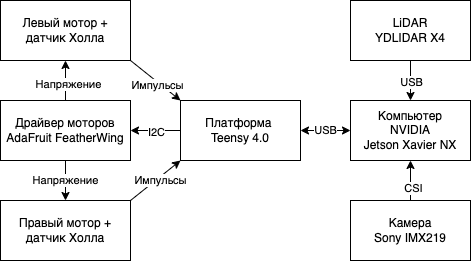
\includegraphics[scale=0.9]{navstack}
    }
    \caption{Общее описание реализованного ROS Navigation Stack}\label{fig:navstack}
\end{figure}

\section{Компоновка оборудования и схема проводки}

Для того чтобы все аппаратные части робота заработали, их нужно обеспечить необходимым питанием. Требуемые напряжения описаны в Таблице~\cref{tab:voltages}.

\begin{table} [htbp]%
    \centering
    \caption{Необходимые напряжения для различных узлов робота}%
    \label{tab:voltages}% label всегда желательно идти после caption
    \renewcommand{\arraystretch}{1.5}%% Увеличение расстояния между рядами, для улучшения восприятия.
    \begin{SingleSpace}
        \begin{tabular}{@{}@{\extracolsep{20pt}}llll@{}} %Вертикальные полосы не используются принципиально, как и лишние горизонтальные (допускается по ГОСТ 2.105 пункт 4.4.5) % @{} позволяет прижиматься к краям
            \toprule     %%% верхняя линейка
            Устройство & Диапазон напряжений \\
            \midrule %%% тонкий разделитель. Отделяет названия столбцов. Обязателен по ГОСТ 2.105 пункт 4.4.5
            Электродвигатели & 9В \\
            Датчики Холла & 5В \\
            Компьютер NVIDIA Jetson Xavier NX  & 9 - 20В \\
            Лазерный сканер YDLiDAR X4 & 5В \\
            Платформа Teensy 4.0 & 5В \\
            Драйвер двигателя Adafruit FeatherWing №2927 &  3.3 В \\
            \bottomrule %%% нижняя линейка
        \end{tabular}%
    \end{SingleSpace}
\end{table}

Исходя из данных требований, а также возможного высокого энергопотребления со стороны компьютера NVIDIA Jetson Xavier NX, было принято решение о покупке мощного аккумулятора TalentCell Rechargeable, который изображён на Рисунке~\cref{fig:battery}. Эта аккумуляторная батарея имеет следующие характеристики~\cite{battery}:

\begin{itemize}[beginpenalty=10000] % https://tex.stackexchange.com/a/476052/104425
  \item Наличие трёх выходных напряжений: 12В, 9В и 5В;
  \item Выходная сила тока: 6А, 1А и 2А соответственно;
  \item Масса 500г;
  \item Размер 79x137x39мм.
\end{itemize}

\begin{figure}[ht]
    \centerfloat{
        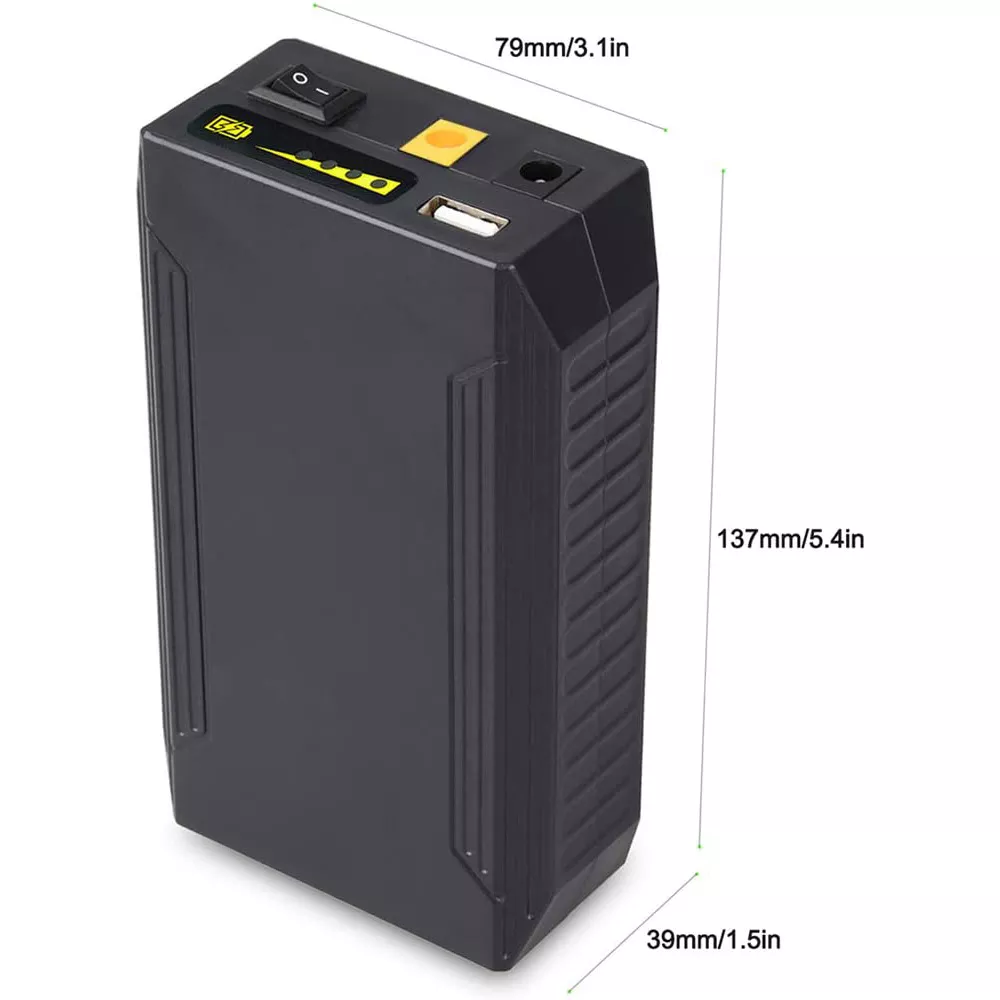
\includegraphics[scale=0.4]{battery}
    }
    \caption{Внешний вид аккумуляторной батареи TalentCell Rechargeable}\label{fig:battery}
\end{figure}

После формирования определённой аппаратной составляющей робота, была составлена схема расположения компонентов на шасси. Схема изображена на Рисунке~\cref{fig:devices}. На верхней части робота расположился компьютер и лазерный сканер, а также камера, которая направлена вперёд. На нижней части находится аккумуляторная батарея, двигатели и драйвер для них, а также платформа Teensy.

\begin{figure}[ht]
    \centerfloat{
        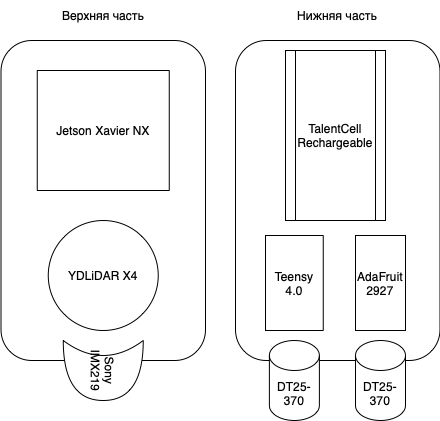
\includegraphics[scale=0.9]{devices}
    }
    \caption{Схема расположения устройств на шасси робота}\label{fig:devices}
\end{figure}

Также была создана схема электропроводки, изображённая на Рисунке~\cref{fig:battery}. При создании электропроводки было учтено, что 5 вольтовый выход с аккумуляторной батареи не является достаточно мощным для обеспечения работы всех устройств, поэтому он использовался исключительно для дополнительного питания YDLiDAR X4. Датчики Холла и платформа Teensy были обеспечены 5 вольтовым напряжением с DC преобразователя с 12 до 5 вольт. Напряжение 3.3В для питания драйвера двигателя также было получено при помощи DC преобразователя с 5 до 3.3 вольт.

\begin{figure}[ht]
    \centerfloat{
        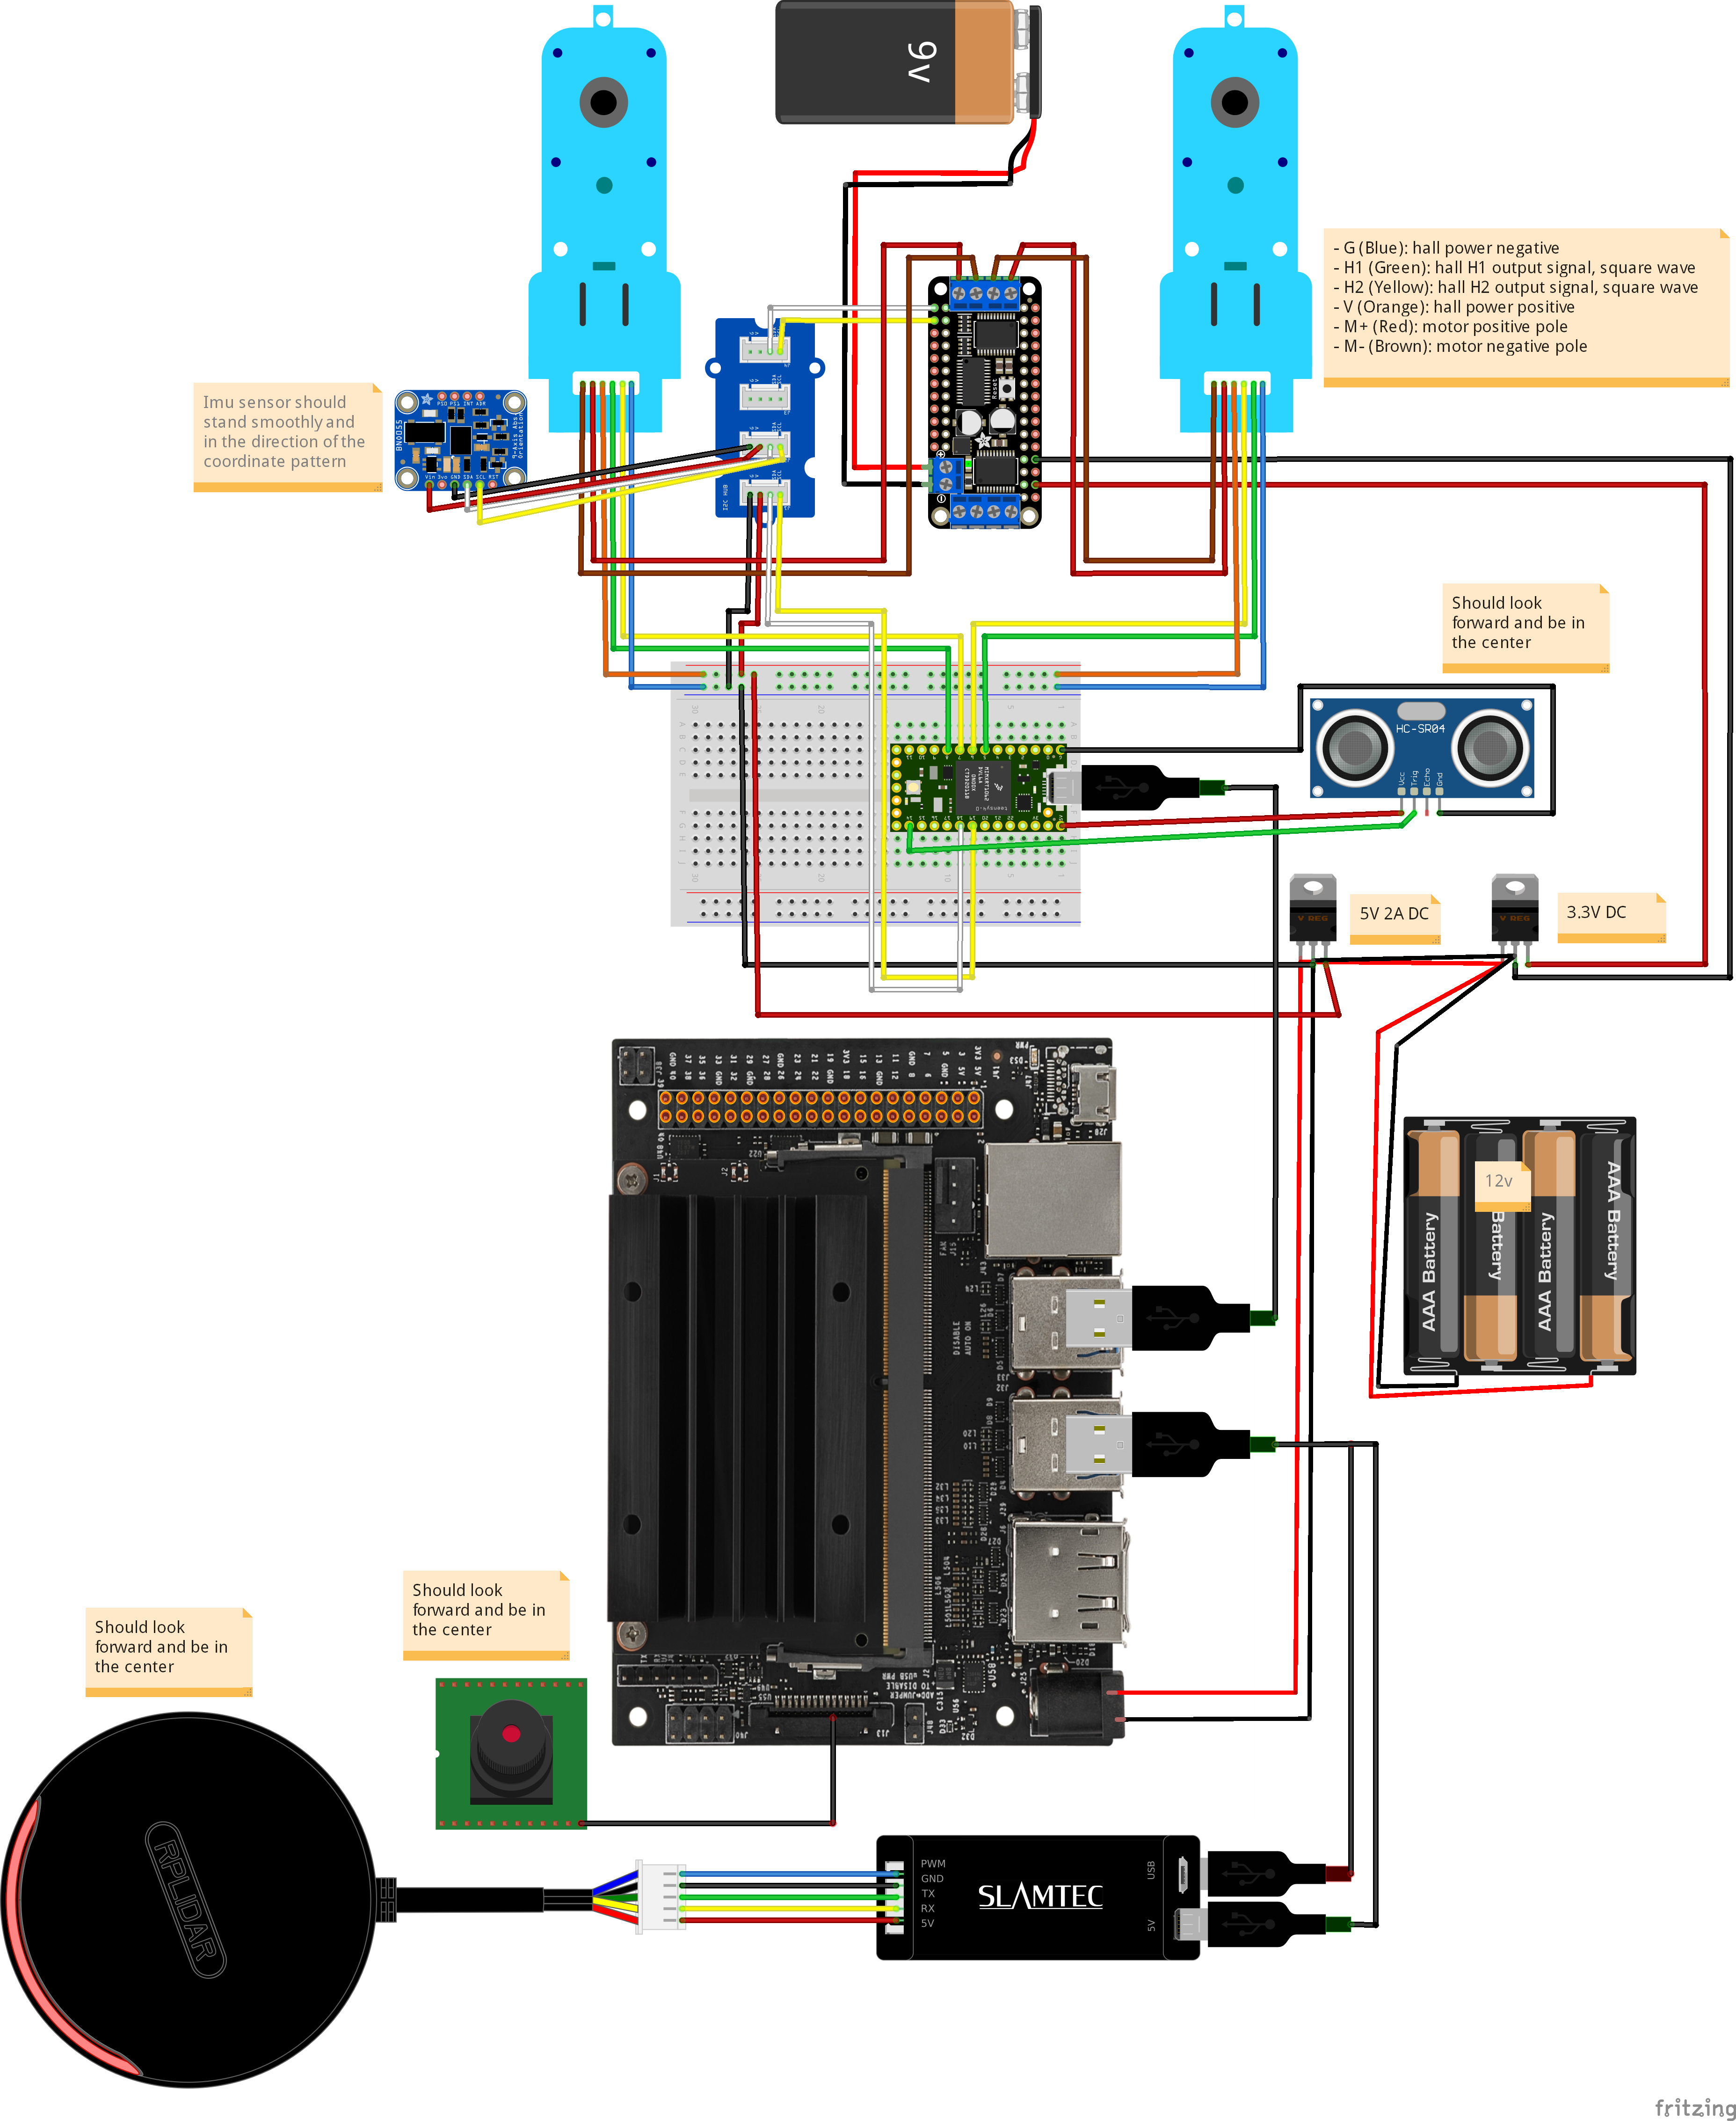
\includegraphics[scale=0.48]{wires}
    }
    \caption{Схема электрической проводки робота}\label{fig:wires}
\end{figure}

\section{Тестирование работоспособности} 
Тестирование работоспособности робота проводилось путём серии экспериментов с ручным и полуавтоматическим управлением.

Суть экспериментов с ручным управлением сводилась к подключению игрового контроллера Sony DualShock 4 к системе ROS посредством пакета <<ds4\_driver>> и самому процессу управления. На данном этапе удалось отладить работу коммуникации компьютера, ПИД-регулятора и выявить неточности, связанные с конфигурациями пакетов, использованных для построения ROS Navigation Stack.

Полуавтоматическое управление роботом предполагает процесс, когда на основе поступивших в него данных и точки, также называемой <<целью>>, робот сам прокладывает маршрут и отправляется в путь. Такой режим управления возможен в частности благодаря таким пакетам, как <<google\_cartographer>>. и <<gmapping>>, который являются реализацией алгоритма SLAM. Пример построенного маршрута в неизвестном пространстве можно увидеть на Рисунке~\cref{fig:path}~\cite{path}. 

\begin{figure}[ht]
    \centerfloat{
        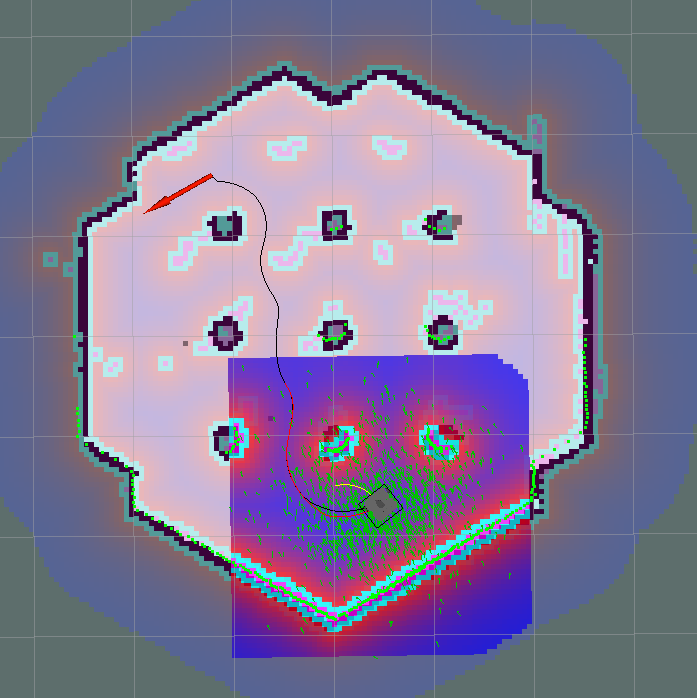
\includegraphics[scale=1.0]{path}
    }
    \caption{Пример картографирования и построения маршрута при помощи SLAM}\label{fig:path}
\end{figure}

Такой процесс можно полностью автоматизировать. Для этого нужно создать алгоритм выбора следующей путевой точки или воспользоваться уже существующим пакетом ROS, который уже решает данную задачу. Этого не было сделано, так как это не является задачей данной работы.

\subsection{Алгоритм SLAM и доступные реализации на ROS}
SLAM - Simultaneous Localization and Mapping или Одновременная Локализация и Картографирование. 

Данный метод навигации используется для определения местоположения и ориентации автономных роботов на заранее неизвестной им местности, а также, для обновления или дополнения уже известных карт окружающего пространства~\cite{slam}. 

Во время тестирования было испробовано 2 реализации SLAM, реализованные в пакетах ROS:

\begin{itemize}[beginpenalty=10000] % https://tex.stackexchange.com/a/476052/104425
  \item GMapping;
  \item Google Cartographer.
\end{itemize}

\subsubsection{GMapping}
GMapping создает карту, благодаря данным LiDAR и одометрии. Как правило, используется 2D LiDAR, подобный тому, что используется в данной работе. Такие LiDAR'ы способны сканировать окружающее пространство в режиме реального времени на 360 градусов. Далее, происходит сопоставление готовой карты, деревьев местоположений Transform и облака точек c LiDAR, в результате чего оценивается и корректируется местоположение робота. Пример построенной карты можно увидеть на Рисунке~\cref{fig:gmapping}~\cite{slam}.

\begin{figure}[ht]
    \centerfloat{
        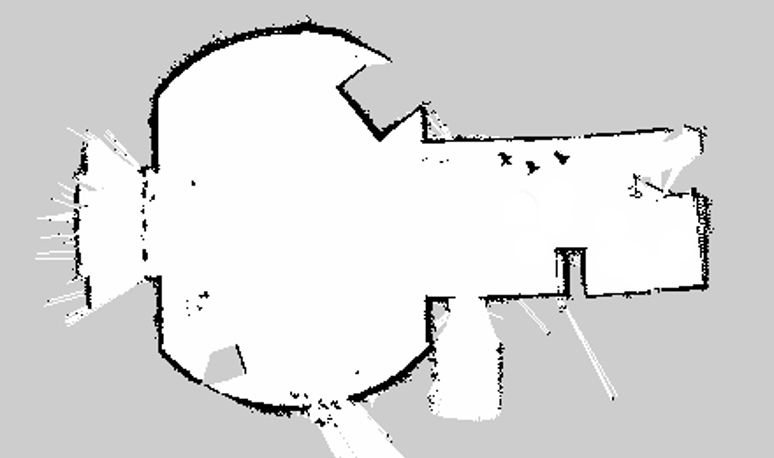
\includegraphics[scale=1.0]{gmapping}
    }
    \caption{Пример визуализации карты, построенной в GMapping}\label{fig:gmapping}
\end{figure}

\subsubsection{Google Cartographer}
Google Cartographer схож с GMapping: он может строить карту по облаку точек с 2D LiDAR'а и данных с одометрии (опционально). Однако, в отличие от GMapping, он обладает намного более богатым функционалом. Например, Cartographer имеет более сложную градацию точек, из которых состоят карты – cells. По мере исследования одного и того же участка местности, Cartographer плавно меняет параметр точек карты с «неизвестно» на «исследовано» с флагом «свободно» либо «препятствие». В результате, Cartographer имеет меньшую вероятность пропустить какие-либо объекты на карте. Пример построения карты данным алгоритмом можно увидеть на Рисунке~\cref{fig:cartographer}~\cite{slam}.

\begin{figure}[ht]
    \centerfloat{
        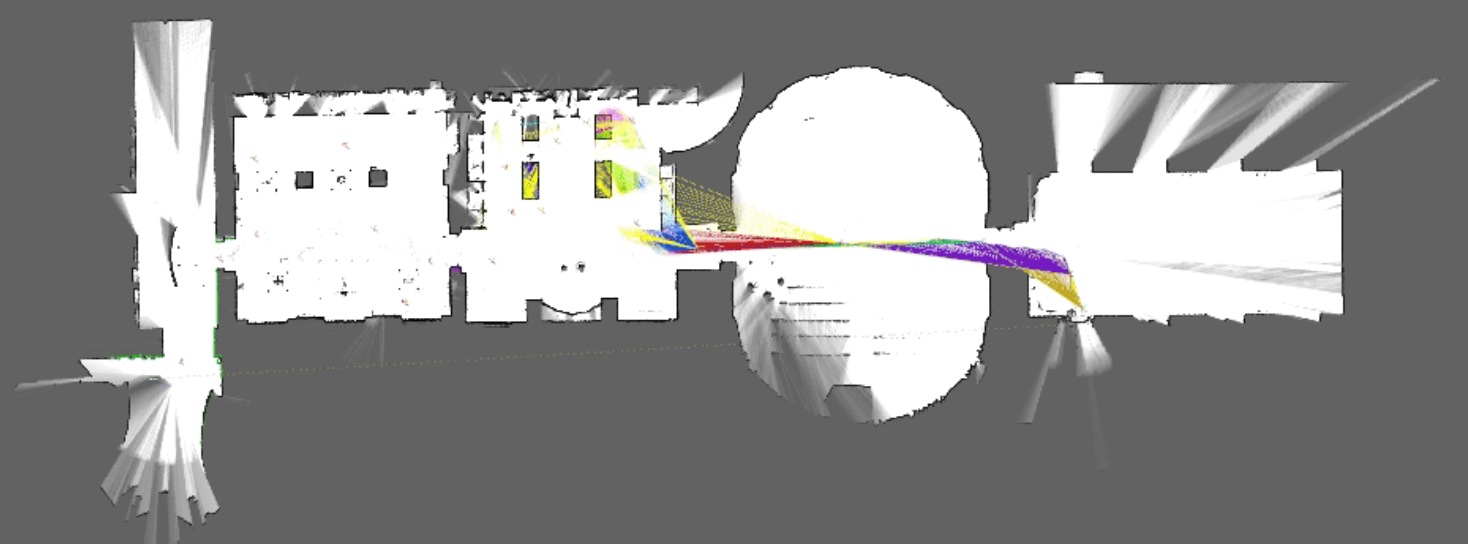
\includegraphics[scale=0.4]{cartographer}
    }
    \caption{Пример визуализации карты, построенной в Google Cartographer}\label{fig:cartographer}
\end{figure}

Каждый из представленных выше алгоритмов имеет свои преимущества и недостатки. К преимуществам GMapping можно отнести его оптимизацию: его реализация алгоритма может без задержек работать на таких одноплатных компьютерах, как Raspberry PI 4B с довольно ограниченным потенциалом вычислительной мощности. К преимуществам Google Cartographer можно отнести более точную локализацию, которая может работать даже без внешнего источника одометрии, используя в качестве входных данных только облако точек LiDAR. Платой за такой функционал является объём вычислений на центральном процессоре устройства, а также высокое потребление оперативной памяти, что и является недостатком Cartographer в сравнении с GMapping.

\section{Сбор тренировочных данных для нейронной сети}
Для сбора необходимых тренировочных данных для нейронной сети использовался стандартный механизм записи и воспроизведения ROS событий - <<rosbag>>. Данная программа позволяет записывать и воспроизводить bag файлы, в которых записаны все данные топиков, событий сервисов, текущее время и т.д. 

Данный формат файлов отлично подходит для записи тренировочных данных нейронной сети по следующим причинам:

\begin{enumerate}[beginpenalty=10000] % https://tex.stackexchange.com/a/476052/104425
  \item Все записанные данные синхронизированы по времени;
  \item Можно записать любые данные при условии, что они публикуются в какой-либо ROS топик; 
  \item Из bag файла можно частями вытаскивать нужные данные, которые легко конвертировать в формат CSV при помощи библиотеки <<bagpy>> для языка программирования Python.
\end{enumerate}

Таким образом было записано несколько bag файлов, которые были использованы в качестве тренировочных данных нейронной сети на основе обучения с подкреплением. В данных файлах содержатся следующие данные: время, местоположение робота относительно включения, облако точек из LiDAR, изображение с камеры, команда на движение. Предполагается, что на записи содержатся действия, которые должны воспроизводиться нейронной сетью. 

\subsection{Описание обучаемой нейронной сети}
Нейронная сеть, которая будет использована для управления роботом работает на базе обучения с подкреплением\footnote{или Reinforcement Learning}. 

При обучении с подкреплением некоторый программный \textbf{агент} делает наблюдения внутри \textbf{среды исполнения}, предпринимает \textbf{действия} и в ответ получает за это \textbf{награды}. Суть такого обучения сводится к методу проб и ошибок: нужно научиться действовать так, чтобы получить максимально возможные награды в долгосрочной перспективе~\cite{reinforcement}. 

Перекладывая, сказанное выше, на разрабатываемую нейронную сеть, это можно описать так: роботом будет управлять \textbf{агент} - нейронная сеть, \textbf{средой выполнения} является замкнутое пространство в котором оказался робот, вооружённый камерой Sony IMX219 и YDLiDAR X4, а \textbf{действиями} будут являться команды на движение на которые подписан узел взаимодействия с драйвером двигателей. Эта система запрограммирована получать положительные награды за нахождение целевых объектов и отрицательные --- за пустую трату времени, а также за близкий подъезд к препятствию.

\subsubsection{Политика действий}
Алгоритм, применяемый программным агентом для определения своих действий, называется политикой. В данном случае политикой будет являться нейронная сеть, которая на входе принимает наблюдение: облако точек и изображение с камеры, а затем выдаёт действие, подлежащее выполнению. Политикой может быть любой алгоритм, какой только можно придумать и в данном случае он не является детерминированным, так как не существует чётких действий к выполнению задачи поиска целевого объекта для всех замкнутых пространств, куда в теории может помещаться робот. 

Схематично обучение политике действий изображено на Рисунке~\cref{fig:act-policy}~\cite{reinforcement}. 

\begin{figure}[ht]
    \centerfloat{
        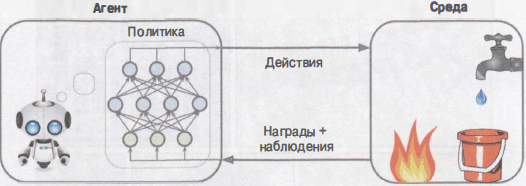
\includegraphics[scale=0.8]{act-policy}
    }
    \caption{Пример обучения с подкреплением, использующего политику в форме нейронной сети}\label{fig:act-policy}
\end{figure}

\subsubsection{Q-обучение}
Q-обучение предполагает, что существуют некие состояния, в которые может переходить робот, а вероятности переходов в эти разные состояния неизвестны. Для каждой пары <<состояние-переход>> ($s, a$) этот алгоритм отслеживает скользящее среднее наград $r$, которые агент получает, когда покидает состояние $s$ посредством действия $a$, плюс наград, которые он ожидает получить позже. Алгоритм Q-обучения описывается уравнением~\cref{eq:q-learn}. Поскольку целевая политика должна действовать оптимально, мы получим максимальные оценки Q-ценностей для следующего состояния.

\begin{equation}
    \label{eq:q-learn}
    Q_{k+1}(s,a)\leftarrow (1-\alpha )Q_{k}(s,a)+\alpha (r+\gamma * \max_{a'}Q_{k}(s',a'))
\end{equation}

\subsection{Мотивация для использования описанной нейронной сети}
Мотивацией для использования описанной выше нейронной сети стали текущие реализации алгоритмов SLAM, которые вычислительно тяжелы, строят карту всего доступного пространства, затем осуществляют привязку робота к этой карте с использованием множества громоздких матричных вычислений. На каждом шаге необходимо пересчитывать карту и выполнять привязку робота заново, что не оптимально. Также алгоритмы SLAM имеют сильную чувствительность к погрешностям работы LiDAR. При выработке управляющих сигналов система может решить, что роботу мешают проехать какие-то препятствия, которые в реальности не существуют и вызваны недостаточной обработкой данных с LiDAR в связи с перерисовкой карты. 

Для того чтобы задать поведение робота, было решено использовать нейронную сеть, которая при создании управляющих сигналов будет учитывать только те точки, которые действительно существуют с учётом фильтра временного усреднения, а также являются достаточно существенными для робота в данный момент. 

Таким образом, робот принимает решения, исходя только из важной информации, которую он <<видит>> перед собой и немного по бокам. Привязка к местности не осуществляется, поскольку главная цель робота - это максимально быстрое нахождение целевого предмета(-ов) и не допущение ситуации, когда робот врезается в препятствие.

Построение карты должно было выполняться отдельным потоком, который предполагалось реализовать после оптимизации управляющей нейронной сети и сети модуля компьютерного зрения. Также, планировалось реализовать механизм <<открытого обучения>>, т.е робот должен был доучиваться в процессе работы, как человек.

\clearpage
